\documentclass[tikz,14pt]{standalone}
\usepackage{textcomp}
\usepackage{amsmath}
\usetikzlibrary{shapes,arrows}
\usetikzlibrary{calc, positioning, plotmarks, shapes.geometric, patterns}
\usetikzlibrary{arrows,automata}

% \newcommand{\isin}{\mathrel{\overset{?}{\in}}}

\begin{document}
% Definition of blocks:
\tikzset{%
  block/.style    = {draw, thick, rectangle, minimum height = 3em,
    minimum width = 3em, node distance=3cm},
  sum/.style      = {draw, circle, node distance = 2cm}, % Adder
  input/.style    = {coordinate}, % Input
  output/.style   = {coordinate} % Output
}

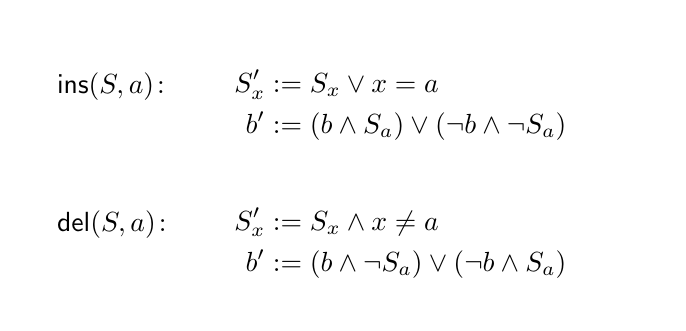
\begin{tikzpicture}[anchor=west]
    \path[use as bounding box, clip] (0,.5) rectangle (8,-3);

    % \begin{scope}[yshift=-0.75cm]

    %   \node (ins_label) at (0.25,0) {$\mathsf{ins}(S, a)\colon$};
    %   \node (ins1) at (2.5,0) {$S'_x := S_x\vee x=a$};
    %   \node (ins2) at (2.645,-0.5) {$b' := (b\wedge S_a)\vee(\lnot b \wedge \lnot S_a) $};
    % \end{scope}
    \begin{scope}[yshift=.5cm]

    \begin{scope}[yshift=-0.75cm]
      \node (ins_label) at (0.25,0) {$\mathsf{ins}(S, a)\colon$};
      \node (ins) at (2.5,-0.25) {%
        $\begin{aligned}
          S'_x &:= S_x\vee x=a \\
          b' &:= (b\wedge S_a)\vee(\lnot b \wedge \lnot S_a)
        \end{aligned}$%
      };
    \end{scope}

    \begin{scope}[yshift=-2.5cm]
      \node (del_label) at (0.25,0) {$\mathsf{del}(S, a)\colon$};
      \node (ins) at (2.5,-0.25) {%
        $\begin{aligned}
          S'_x &:= S_x \wedge x\neq a \\
          b' &:= (b\wedge \lnot S_a)\vee(\lnot b \wedge S_a)
        \end{aligned}$%
      };
    \end{scope}

    % \begin{scope}[yshift=-2.5cm]
    %   \node (del_label) at (0.25,0) {$\mathsf{del}(S, a)\colon$};
    %   \node (del1) at (2.5,0) {$S'_x := S_x \wedge x\neq a$};
    %   \node (del2) at (2.645,-0.5) {$b' := (b\wedge \lnot S_a)\vee(\lnot b \wedge S_a) $};
    % \end{scope}

    \end{scope}

\end{tikzpicture}
\end{document}